\documentclass[11pt,a4paper,oneside]{report}
\usepackage[ngerman]{babel}
% \usepackage{url} or
\usepackage[utf8]{inputenc} % Displays German 'Umlaute' correctly. Also some workaround, see Bibliography Management#BibTeX in wikibooks
\usepackage{graphicx}
%\usepackage{titlesec}
\usepackage{hyperref}
\usepackage{chngcntr}

\setcounter{secnumdepth}{3}
\setcounter{tocdepth}{5}

% Enables consecutive figure and table numbering, independent of chapter count
\counterwithout{figure}{chapter}
\counterwithout{table}{chapter}

\addto{\captionsngerman}{\renewcommand*{\abstractname}{Abstract}}
%\renewcommand{\abstractname}{Abstract}

\newcommand{\bibtexFilename}{draft} % written without extension
\newcommand{\thema}{Sicherheitsbetrachtungen von Applikations-Containersystemen in Cloud-Infrastukturen am Beispiel Docker}
\newcommand{\fig}{Abb.}
\newcommand*{\signatureAndDate}{
    \par\noindent\makebox[2.5in]{\hrulefill} \hfill\makebox[2.0in]{\hrulefill}%
    \par\noindent\makebox[2.5in][l]{Unterschrift}      \hfill\makebox[2.0in][l]{Datum}%
}

\begin{document}
\pagenumbering{gobble} % No page numbers

\begin{titlepage}
	\centering
	% \includegraphics[width=0.15\textwidth]{example-image-1x1}\par\vspace{1cm}
	{\scshape\LARGE
		Hochschule der Medien
	\par}
	\vspace{1cm}
	{\scshape\Large
		Bachelorarbeit
	\par}
	\vspace{1.5cm}
	{\huge\bfseries
		\thema
	\par}
	\vspace{2cm}
	{\Large\itshape
		Moritz Hoffmann
	\par}
	\vspace{0.5cm}
	{\Large
		Studiengang: Mobile Medien\\
		Matrikelnummer: 26135\\
		E-Mail: \texttt{mh203@hdm-stuttgart.de}
	\par}
	\vspace{1.5cm}
	{\Large Dezember 2015\par}
	% Bottom of the page
	\vfill
	{\Large
		\emph{Erstbetreuer:}\hfill\emph{Zweitbetreuer:}\\
		Prof. Dr. Joachim Charzinski\hfill Patrick Fröger\\
		Hochschule der Medien\hfill ITI/GN, Daimler AG
	\par}

\end{titlepage}


\title{\thema}
\author{Moritz Hoffmann\\
  Studiengang Mobile Medien,\\
  Hochschule der Medien\\
  \texttt{mh203@hdm-stuttgart.de}}
\date{Dezember 2015}
% \date{\today}
\maketitle

%\pagenumbering{roman}

\chapter*{Eidesstattliche Erklärung}
\emph{„Hiermit versichere ich, Moritz Hoffmann, ehrenwörtlich, dass ich die vorliegende Bachelorarbeit mit dem Titel: „\thema“ selbstständig und ohne fremde Hilfe verfasst und keine anderen als die angegebenen Hilfsmittel benutzt habe. Die Stellen der Arbeit, die dem Wortlaut oder dem Sinn nach anderen Werken entnommen wurden, sind in jedem Fall unter Angabe der Quelle kenntlich gemacht. Die Arbeit ist noch nicht veröffentlicht oder in anderer Form als Prüfungsleistung vorgelegt worden. Ich habe die Bedeutung der ehrenwörtlichen Versicherung und die prüfungsrechtlichen Folgen (§26 Abs. 2 Bachelor-SPO (6 Semester), § 24 Abs. 2 Bachelor-SPO (7 Semester), § 23 Abs. 2 Master-SPO (3 Semester) bzw. § 19 Abs. 2 Master-SPO (4 Semester und berufsbegleitend) der HdM) einer unrichtigen oder unvollständigen ehrenwörtlichen Versicherung zur Kenntnis genommen.“
}
\vspace{1.5cm}
\signatureAndDate
\newpage


% Abstract
\begin{abstract}
\noindent\emph{English version:}\newline\newline
\noindent
....\\
..\\

\vspace{1cm}
\noindent\emph{Deutsche Version:}\newline\newline
\noindent
....\\
...\\
.\\
..\\

\end{abstract}

% Table of Contents
\tableofcontents

% Abbildungsverzeichnis
\listoffigures

% Tabellenverzeichnis
\listoftables

% \linespread{1.3}            % 1.5x line spacing
% \linespread{1.6}            % Double line spacing
% \hfill test                 % insert horizontal stretched space
% \vfill test                 % insert vertical stretched space
% ,,German quotation marks``  % deutsche Anfuehrungszeichen

% this is a comment
Hallo %\cite{myquote1}
One more line %\cite[S.2]{myquote1,myquote2}
jooooo \cite{presContainerDockerSec}

\begin{figure}[h] % with [p], images is displayed on own page
    \centering
    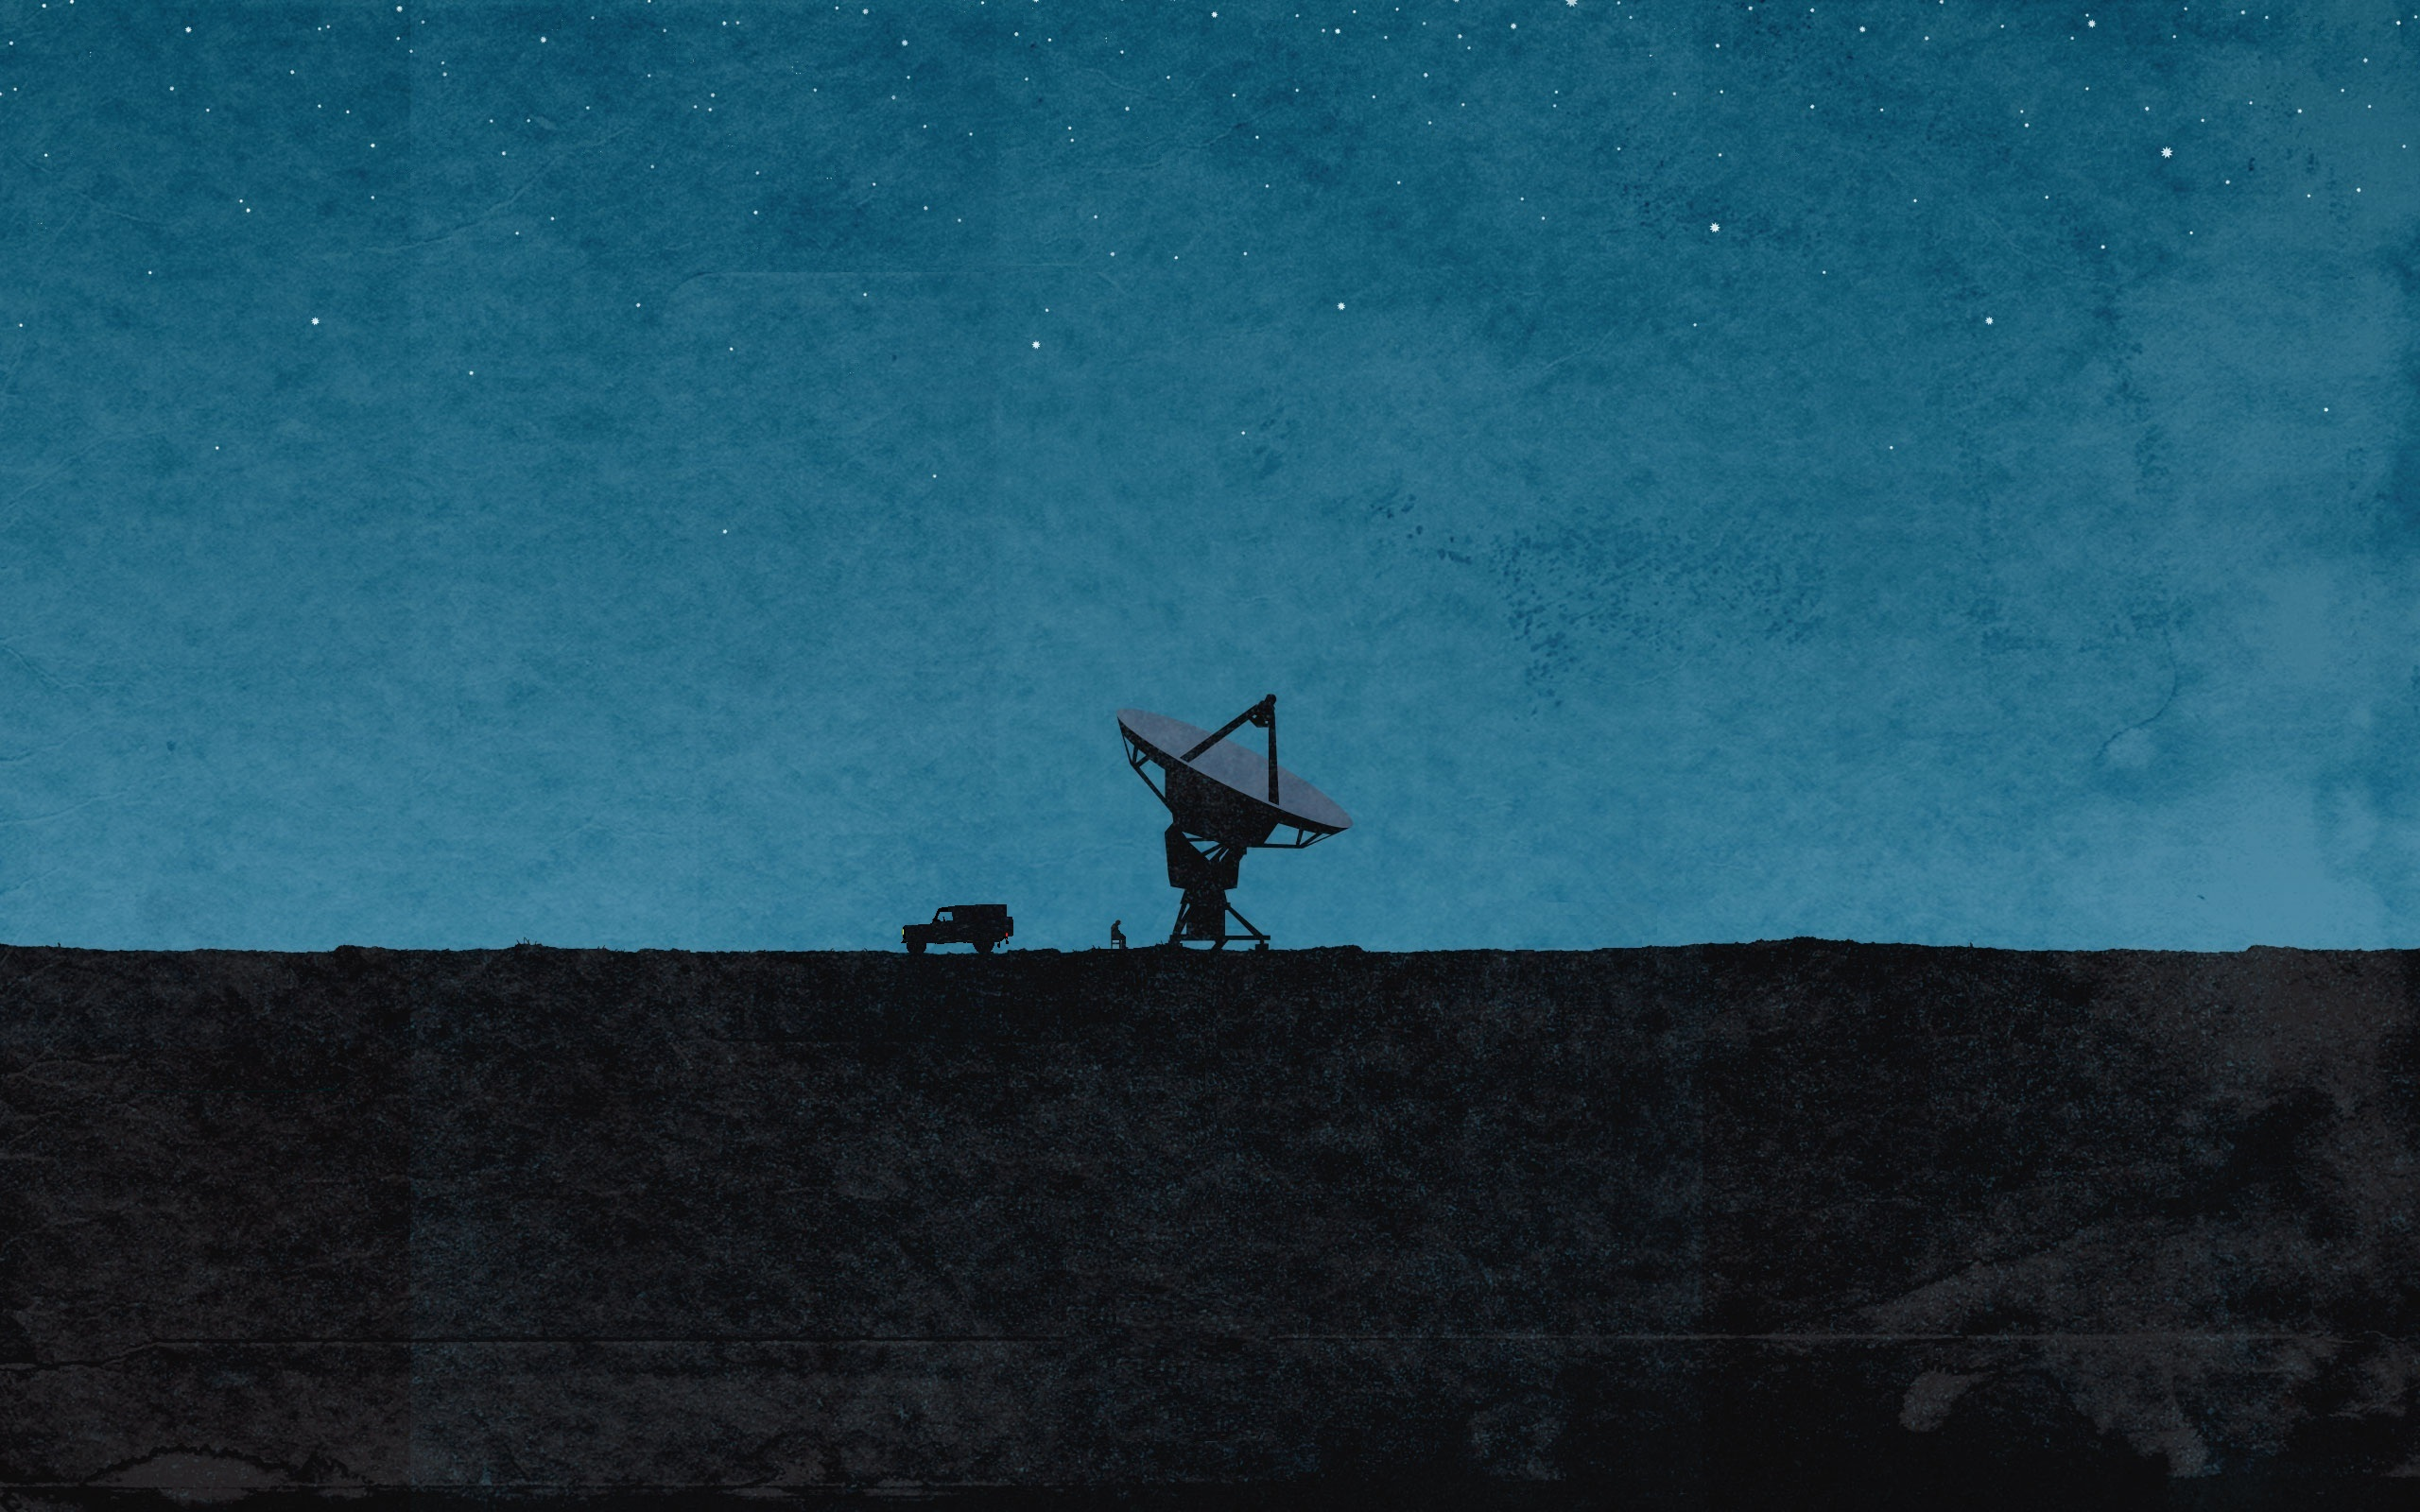
\includegraphics[width=1.0\textwidth]{./images/image.jpg}
    \caption{Awesome Image}
    \label{fig:awesome_image}
\end{figure}

lkasjdflkj asldkjf lasjkdflkadsjf ladksjflkjslkdjf    dslfjklaks df a sdfjaldsfj  ladksjf lkjlakjsd f asdf aljsdflkjasldfjalsdfj l adskjflj d f dslkfjalksdjf sd fljsdfkjsld f

\emph{dieser text ist kursiv}

asdfasdfasdfasdlkvalrkgjval  asdkfj  sldkfjlsdjfa adaher is kes ji lkaskdj ladskj a ldksfjll aldkfj lkj afsdlfkjl alsdkf jaldskfj la sdflaldsflas df sadfl sf

\texttt{das hier ist monotype}

% TODO: reformat chapter style with package titlesec
%\titleformat{\section}
%{\filcenter\normalfont\Large\bfseries}
%{\chaptertitlename~\thechapter} {0.5em} {}



% GLIEDERUNG
\chapter{Überblick}
\pagenumbering{arabic}
  % Container als leichtgewichtige Virtualisierung

  Trotz ein paar intrinsischen Schwächen von Containerlösungen, werden Container bereits in einer Vielzahl von Szenarien eingesetzt \cite[S.6]{dockerBook}.

  Container sind in Infrastrukturen, in denen es auf Skalierbarkeit ankommt, trotz Sicherheitsbedenken beliebt. Vor allem "Multi-Tenant" Services werden gerne mit Docker eingesetzt.
	\section{Arten von Virtualisierungen}
    % AUCH: Vergleich von Virtualisierungsarten
    \subsection{Hypervisor-basierte Virtualisierung}
      Bei Hypervisor-basierten Systemen laufen unabhängig voneinander eine oder mehrere Maschinen virtuell auf physischer Hardware (in der englischen Literatur auch "bare metal" genannt). Der Hypervisor nimmt dabei die Rolle eines Vermittlers zwischen Host-OS und Gast-OS ein \cite[S.6]{dockerBook}.
    \subsection{Container-basierte Virtualisierung}
      (Benötigt keine Emulations- oder Hypervisorschicht \cite[S.7]{dockerBook}.)

      Container-Virtualisierung wird oftmals Virtualisierung auf Betriebsystemebene genannt \cite[S.6]{dockerBook}.

      Containerlösungen umfassen die Technologien \emph{OpenVZ}, \emph{Solaris Zones}, sowie Linux-Container wie \emph{LXC} \cite[S.7]{dockerBook} und \emph{Docker}, welches im Fokus dieser Arbeit steht.

      Moderne Container können als vollwertige Systeme betrachtet werden, nicht mehr als ursprünglich vorgesehen, reine Ausführungsumgebungen \cite[S.7]{dockerBook}.

      In Container-basierten Systemen hingegen, laufen die Container im "User Space" direkt auf dem Kernel des Host-OS und nutzen dessen \emph{System Call}-Interface \cite[S.6+7]{dockerBook}. Dadurch kommt es im Vergleich zu Hypervisor-Virtualisierungen zu einem erheblichen Performancegewinn, da der Virtualisierungs-Overhead des Hypervisors wegfällt. In der Praxis macht das eine hohe Dichte an Containern auf einem Host und dadurch indirekt eine bessere Resourcenausnutzung möglich \cite[S.7+8]{dockerBook}.

      Container-Lösungen erlauben es, mehrere voneinander isolierte "User Space"-Instanzen parallel auf einem einzigen physischen Host zu betreiben \cite[S.6]{dockerBook}. Dadurch, dass ein Hypervisor in einer solchen Konfiguration nicht existiert und die Container direkt Hostkernel-Features nutzen, gibt es einen entscheidenden Nachteil für Containerlösungen - und damit auch Docker - gegenüber Hypervisor-basierter Virtualisierung: Das Container-Betriebssystem muss wie das Host-Betriebsystem Linux-basiert sein. In einem Host auf dem Ubuntu Server installiert ist, können nur weitere Linux-Distributionen als Container laufen. Ein Microsoft Windows kann also nicht als Container auf genannten Host gestartet werden, da die Kernel miteinander nicht kompatibel sind \cite[S.6]{dockerBook}. Diese Inflexibilität im Spektrum der einsetzbaren Betriebssysteme liegt den Containerlösungen zugrunde.

      Außerdem werden Container als weniger sicher im Vergleich zur Hypervisor-gestützen Virtualisierung gesehen \cite[S.6]{dockerBook}.

      Hingegen muss in containerbasierten Systemen nicht das gesamte Betriebssystem virtualisiert werden, da von den Containern direkt auf den Host-Kernel zugegriffen wird. Zum Einen schrumpft dadurch die Angriffsfläche des Hosts \cite[S.6]{dockerBook}, da, wie später noch zu sehen ist, die Zugriffsrechte der Container auf den Host sehr feingranular festgelegt werden müssen. Zum Anderen entsteht durch diese Tatsache ein Risko im Design, weil Host-Features ohne Hypervisor direkt genutzt werden.
	  \subsection{Einordnung Docker}
      Docker nutzt moderne Linux-Kernelfeatures, wie z.b. \emph{control groups} und \emph{namespaces}, um ein Resourcenmanagement zwischen Containern und eine effektive Isolierung der Container vom Hostsystem zu realisieren \cite[S.7]{dockerBook}.

      Docker ist wie in KAPITEL-ZUVOR angedeutet, nicht die erste containerbasierte Virtualisierungslösung. Einige ältere Containersysteme, wie z.B. \emph{Solaris Zones}, gibt es schon viel länger als Docker, aber wurden allerdings nie von der Industrie als Lösung akzeptiert. Worauf beruht also der Erfolg von Docker in den letzten Jahren? Dieser Frage werde ich im folgenden Kapitel nachgehen.
  \section{Einführung in Docker}
    Docker ist eine unter der Apache 2.0 Lizenz veröffentlichte Open-Source Engine, die den Einsatz von Anwendungen in Containern automatisiert. Es ist überwiegend in der Programmiersprache \emph{Golang} von dem Unternehmen \emph{Docker, Inc.} (vormals \emph{dotCloud Inc.}), implementiert \cite{githubDocker}\cite[S.7]{dockerBook}.

    % Erfolg von Docker von businessinsiders.com trends.
    % --> siehe Quelle slideshareDockercon15
    % Auch checken: Statistika, google trends


    Der große Vorteil von Docker gegenüber älteren Containerlösungen ist das Level an Abstraktion und die Bedienungsfreundlichkeit, die Nutzern ermöglicht wird. Während sich Lösungen vor Docker auf dem Markt durch deren schwierige Installation und Management sowie schwachen Automatisierungsfunktionen nicht etablieren konnten, addressiert Docker genau diese Schwachpunkte \cite[S.7]{dockerBook} und bietet neben Containern viele Tools, die die Arbeit mit Containern und weiteren Modulen, erleichtern.

    Quellcode kann samt virtualisierter Ausführungsumgebung flexibel von einem Laptop auf einen Testserver und später auf einen Produktionsserver geschoben werden. Dieser kurzlebige Zyklus zwischen Entwicklung, Testen und Deployment erlaubt einen effizienten Workflow \cite[S.8]{dockerBook}.

    % Einfaches "Getting Started": es braucht nur einen minimalen Host mit einem kompatiblen Linux-Kernel und die Docker-Binary, die ausgeführt werden soll \cite[S.8]{dockerBook}.

    Eine weitere wichtige Eigenschaft von Docker ist Konsistenz: Die Umgebungen, in denen Softwareentwickler Code schreiben, sind identisch mit den Umgebungen, die später auf Servern laufen. Die Wahrscheinlichkeit, dass ein Fehler erst im Betrieb auftritt, nicht aber in der Entwicklung, wird dadurch sehr klein gehalten \cite[S.8]{dockerBook}.

    Wenn wie von Docker empfohlen in jedem Container nur eine Anwendung läuft, begünstigt das eine moderne Service-orientierte Architektur mit \emph{Microservices}. Nach dieser Architektur werden Anwendungen oder Services verteilt zur Verfügung gestellt und durch eine Serie an miteinander kommunizierenden Containern umgesetzt. Der Grad an Modularisierung der dadurch ensteht, kann für die Verteilung, die Skalierung und das Debugging von Service- oder Anwedungskomponeten (Container) gewinnbringend eingesetzt werden \cite[S.9]{dockerBook}.

    Die Eigenheiten von Docker sowie die gängige Begrifflichkeiten im Docker-Ökosystem, werden in den folgenden Unterkapiteln genauer beleuchtet.
    \subsection{Container}
      Der Begriff \glqq{}Container\grqq{} ist bisher schon oft gefallen, deswegen will ich auf ihn zuerst eingehen.

      Docker-Container beinhalten eine idealerweise minimale Laufzeitumgebung, in der eine oder mehrere Anwendungen laufen.

      Basiert auf einem \emph{Copy-on-write}-Modell, das Änderungen der Anwendung schnell handhabt \cite[S.8]{dockerBook}.
      % Copy-on-write erklären.
    \subsection{Images}
    \label{dockerImages}
      Images liegen Containern als statische Files zugrunde. Container werden auf der Basis von Images gestartet. Images sind durch das eingesetzte \emph{Union-Filesystem} in Schichten gegliedert, die zusammen ein Image ergeben, das als Container gestartet werden kann \cite[S.11]{dockerBook}.

      % Screenshot von Imagelayer.io, um Aufbau von einem Image zu sehen

      % Screenshot von docker ps / docker history um Liste von Images zu sehen.
      % Images bekommen einen eindeutigen Hashwert zugewiesen, lassen sich



      Images werden Schritt für Schritt erstellt, z.B. mit den folgenden Aktionen \cite[S.11]{dockerBook}:
      \begin{itemize}
        \item Eine Datei hinzufügen
        \item Ein Kommando ausführen, z.B. ein Tool mittels des Paketmanagers \texttt{apt} installieren
        \item Einen Port öffnen, z.B. den Port 80 für einen Webserver
      \end{itemize}

      Images sind einfach portierbar und können geteilt, gespeichert und aktualisiert werden \cite[S.11]{dockerBook}.

      Auf der Basis von existierenden Images können durch das Hinzufügen neuer Schichten durch oben beschriebene Aktionen, neue Images erstellt werden (EIGENES STATEMENT).

      Über die Kommandozeile kann z.B. das Image eines \emph{Nginx}-Webservers von der öffentlichen Docker-Registry mit dem Befehl \texttt{docker pull nginx} auf die lokale Maschine gespeichert werden.

      %Was eine Registry ist wird im folgenden Kapitel erklärt.

    \subsection{Registries}
      Docker stellt eine Vielzahl an Images öffentlich in einer eigenen Registry, dem Docker Hub \cite[S.11]{dockerBook}, zur Verfügung. Für dieses System kann jeder Nutzer einen Account anlegen und eigenständig Images hochladen. Das Docker-Hub bietet bereits mehr als 150.000 Repositories, die etwa 240.000 Nutzer zusammenstellten und hochluden, zur freien Verwendung an (Stand Juni 2015) \cite[S.16]{slideshareDockercon15}. Die Einträge im Hub können von Nutzern bewertet werden. Außerdem wird angezeigt, wie oft ein Image bereits über das Hub bezogen wurde.

      Ein Repository besteht aus mindestens einem Image. Um Images in einem Repository voneinander zu unterscheiden, werden Images Tags zugewiesen, um beispielweise mehrere Versionen eines Images in einem Repository zu kennzeichnen. Die Images werden nach dem Schema \texttt{<repository>:<tag>} identifiziert. So gibt es z.B. im offiziellen Repository des Webservers \emph{Nginx} Images mit den Tags \texttt{latest}, \texttt{1}, \texttt{1.9} und \texttt{1.9.9} \cite{dockerhubNginx}. Wenn bei dem Download kein Tag angegeben ist, wie in Kapitel wird automatisch das aktuellste Image \texttt{latest} bezogen, wie es im \hyperref[dockerImages]{letzten Kapitel \glqq{}Images\grqq{}} praktiziert wurde.

      % es gibt eine Trusted Registry. Die noch erklären.

      % Bsp. geben für z.B. Ubuntu mit vielen Unterversionen und dem Identifier "latest".

      % Weitere beispiele aus dockerBook: Nginx web server, MySQL Datenbank

      % Es gibt offizielle Images, die von trusted parties verwaltet werden
    \subsection{Dockerfile}


    \subsection{Client und Server}
      Docker selbst ist nach einem Client-Server-Modell aufgebaut: Ein Docker-Client kommuniziert mit einem Docker-Daemon, also ein Prozess der den Server abbildet. Beide Teile können auf einer Maschine oder einzeln auf unterschiedlichen Hosts laufen. Wie in \fig \ref{fig:intro_dockerArchitecture} zu sehen ist, sind auch mehrere Docker-Clients möglich.
      % in beiden Fällen wird eine RESTful API genutzt? Setzt das docker binary nur CLI-Kommandos in REST-API-Aufrufe um?
      % Docker-Binary \texttt{docker}

      \begin{figure}[h]
          \centering
          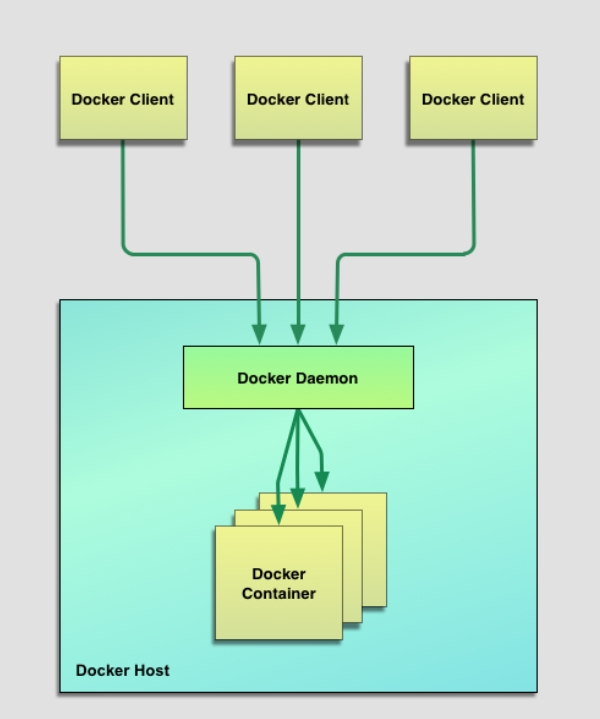
\includegraphics[width=0.7\textwidth]{./images/intro_dockerArchitecture.jpg}
          \caption{Die Client-Server-Architektur von Docker \cite[S.10]{dockerBook}.}
          \label{fig:intro_dockerArchitecture}
      \end{figure}

      % Kommunikation zwischen Client und Server via TCPIP oder Unix Sockets?

\chapter{Ziel der Arbeit/Forschungsfrage}
  % Kommt man von Container auf Host-OS? Von Container auf anderen Container? ~etc.
  % 5-6 Sicherheitsziele erwähnen. Mit Forschungsfrage in Bezug bringen --> später bei Isolierung und Ressourcenverwaltung wieder aufgreifen
\chapter{Security aus Linux Kernel-Features}
  % namespaces/etc (was es ist) in Einleitung mit rein? 1.) Erklaeren, 2.) Security/Docker untersuchen dazu im Security Hauptteil
  % 2 Unterkapitel, inhatliche Überschneidung evtl., Grund nennen warum so gegliedert, ...
	\section{Isolierung}
    % Isolierung erklären, erfüllt X Schutzziele, Bezug auf Forschungsfrage
		\subsection{\texttt{namespaces}}
			\subsubsection{\texttt{user namespaces}}
      % Future implementation, da sehr neu. Trotzdem Konzept erklären und wie Docker-Security davon profitiert.
		\subsection{\texttt{capabilities}}
			\subsubsection{Beispiele, \texttt{/proc}-Verzeichnis, (Un-)Mounten des Host-Filesystems}
      % Gehört das unter 'capabilities'? Oder eigener Punkt bzw. woanders dazu?
		\subsection{Mandatory Access Control (MAC)}
      % Herausfinden, ob das wirklich Unterkapitel von "Isolierung" wird. Evtl. getrennt davon listen.
			\subsubsection{Beispiel SELinux}
      % Macht Sinn das erst am Ende zu machen, wenn noch Zeit ist. Weil SELinux im Detail mehr Exkurs wird.
      \subsubsection{AppArmor}
      % Optional, da auf MAC alzu sehr eingehen nicht zu sehr im Scope sein sollte.
	\section{Ressourcenverwaltung}
    % Sicherheitsziel: Availability, Bezug auf Forschungsfrage
    % Ressourcenverteilung und -management
    % Storage, CPU, HDD, RAM, IO, Network
		\subsection{\texttt{cgroups}}
	\section{Docker im Vergleich zu anderen Containerlösungen}
  % Optional?
\chapter{Security im Docker-Ökosystem}
  % ### Hier mit Patrick weitermachen ###
  % Je nach Vorankommen, können hier ganze Sektions weggelassen werden imo.
  % Tendenziell mehr die Themen zuerst, die direkt mit Security zu tun haben.
  % Auch Fokus auf die neusten Entwicklungen (2015 und 2016) in Sachen Sicherheit und neue Docker-Features
  \section{Docker Images und Registries}
    % Siehe /cite{slideshareDockercon15}, slide 51
		\subsection{neues Signierungs-Feature}
	\section{Docker Daemon}
		\subsection{REST-API}
		\subsection{Support von Zertifikaten}
  \section{Containerprozesse}
    % offenbar gibts Probleme mit PID=0, da dieser Besonderheiten aufweist (siehe Hackernews Link)
	\section{Docker Cache}
	\section{\texttt{privileged} Container}
	\section{Networking}
		\subsection{\texttt{bridge} Netzwerk}
		\subsection{\texttt{overlay} Netzwerk}
		\subsection{DNS}
		\subsection{Portmapping}
	\section{Daten-Container}
	\section{Docker mit VMs}
  \section{Sicherheitskontrollen für Docker}
    % Gibt auf Github Skripte, die einige Docker-Parameter/Einstellungen prüfen (Links iwo in den Bookmarks)
	\section{Tools rund um Docker}
		\subsection{Docker Swarm}
		\subsection{Docker Compose}
		\subsection{Nautilus Project}
		\subsection{Vagrant}
		\subsection{Kubernetes}
      % neueres Cluster-Management Tool von Google
      % Hat Relevanz fuer Herr Fahner/Daimler
\chapter{Docker in Unternehmen/Clound-Infrastrukturen}
  % Wichtiges Kapitel für Daimler, mein Chef, Management
  % Kapitel, das erst angegangen wird, wenn min. Kapitel 1 steht (Januar 2016 oder später).

  % ???: Transscript aus Besprechung mit Herr Fahner und Patrick:
  % Welche Security-Features uebernimmt die Cloud, welche muss Docker gewaehrleisten. Was
  % bieten MS Azure/Amazon's AWS/etc fuer Mechanismen an?
  % Welche Möglichkeiten zur sicheren Docker-Integration bieten diese?
  % Wortlaut Patrick: Wie funktionierts bei Azure, wie funktionierts wenn man es
  % selbst implementiert.

  % --> mir ist nich klar, was ich da untersuchen kann.
\chapter{Fazit/Ausblick}
  % Wenig Angriffsvektoren auf Docker/Container bekannt. "Sichergehen" kann man nur mit Konzepten wie "Docker in VMs" und "VMs in Docker".
  % neuste Docker-Releases und deren Fokus (Enterprise,Production-Readiness,Security)
  % seit Juli 2015 ist standardisiertes Containerformat der big player in Arbeit
  % Ausblick im Kontext von Container VS. konventioneller Virtualisierung


%\subsection{Subsektion blabla}
%\subsubsection{Subsubsektion blablabla}
%\paragraph{Paragraph soundso}
%\subparagraph{SubParagraph soundso}

% Anhang
\appendix
  % Falls benoetigt
  % Evtl. beispielhafte Dockerfiles anzeigen

% Bibliography
\bibliographystyle{plain}
\bibliography{\bibtexFilename} % specify name of bibfile

\end{document}
